%\documentclass[tikz, border=5mm]{standalone}

\usetikzlibrary{arrows,shadows,positioning}

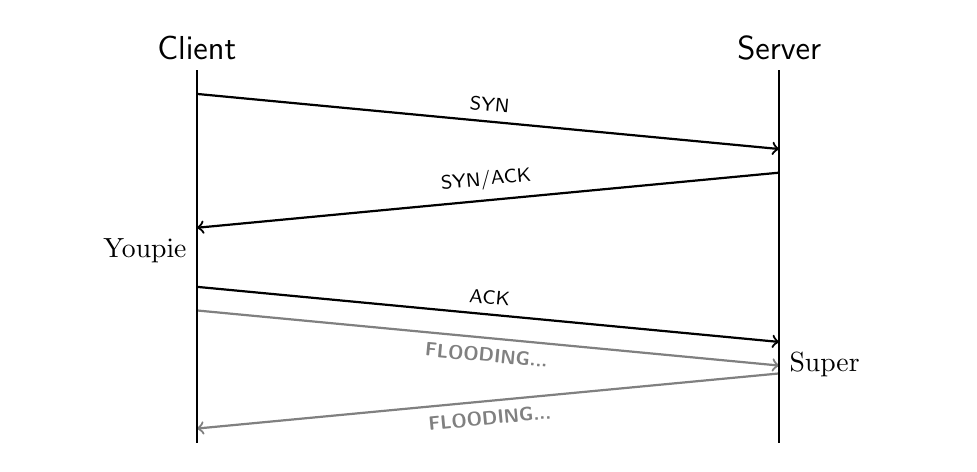
\begin{tikzpicture}[font=\sffamily,thick,
commentl/.style={text width=1.9cm, align=right},
commentr/.style={commentl, align=left},]
\node[] (init) {\large Client};
\node[right=6.1cm of init] (recv) {\large Server};


\draw[->] ([yshift=-0.3cm]init.south) coordinate (syn1o) -- ([yshift=-.7cm]syn1o-|recv) coordinate (syn1e) node[pos=.5, above, sloped] {\scriptsize SYN};

\draw[->] ([yshift=-0.3cm]syn1e) coordinate (synack1o) -- ([yshift=-.7cm]synack1o-|init) coordinate (synack1e) node[pos=.5, above, sloped] {\scriptsize SYN/ACK};

\node[commentl, below left =0mm of synack1e, font=\fontsize{9pt}{9pt}\biolinum]{Youpie};

\draw[->] ([yshift=-.75cm]synack1e) coordinate (ack1o) -- ([yshift=-.7cm]ack1o-|recv) coordinate (ack1e) node[pos=.5, above, sloped] {\scriptsize ACK};

\node[commentr, below right =0mm of ack1e, font=\fontsize{9pt}{9pt}\biolinum]{Super};

%\draw[->] ([yshift=-.4cm]ack1e) coordinate (ack2o) -- ([yshift=-.7cm]ack2o-|init) coordinate (ack2e) node[pos=.5, above, sloped] {\scriptsize ACK};
\draw[gray,->] ([yshift=-.3cm]ack1o) coordinate (data1o) -- ([yshift=-.3cm]ack1e) coordinate (data1e) node[pos=.5, below, sloped] {\scriptsize \textbf{FLOODING...}};

\draw[gray,->] ([yshift=-.4cm]ack1e) coordinate (data2o) -- ([yshift=-.7cm]data2o-|init) coordinate (data2e) node[pos=.5, below, sloped] {\scriptsize \textbf{FLOODING...}};

\node[below =4.5cm of init](end){};

\draw[thick, shorten >=-.1cm] (init) -- (init|-end);
\draw[thick, shorten >=-.1cm] (recv) -- (recv|-end);
\end{tikzpicture}